%% bare_conf.tex
%% V1.4b
%% 2015/08/26
%% by Michael Shell
%% See:
%% http://www.michaelshell.org/
%% for current contact information.
%%
%% This is a skeleton file demonstrating the use of IEEEtran.cls
%% (requires IEEEtran.cls version 1.8b or later) with an IEEE
%% conference paper.
%%
%% Support sites:
%% http://www.michaelshell.org/tex/ieeetran/
%% http://www.ctan.org/pkg/ieeetran
%% and
%% http://www.ieee.org/

%%*************************************************************************
%% Legal Notice:
%% This code is offered as-is without any warranty either expressed or
%% implied; without even the implied warranty of MERCHANTABILITY or
%% FITNESS FOR A PARTICULAR PURPOSE! 
%% User assumes all risk.
%% In no event shall the IEEE or any contributor to this code be liable for
%% any damages or losses, including, but not limited to, incidental,
%% consequential, or any other damages, resulting from the use or misuse
%% of any information contained here.
%%
%% All comments are the opinions of their respective authors and are not
%% necessarily endorsed by the IEEE.
%%
%% This work is distributed under the LaTeX Project Public License (LPPL)
%% ( http://www.latex-project.org/ ) version 1.3, and may be freely used,
%% distributed and modified. A copy of the LPPL, version 1.3, is included
%% in the base LaTeX documentation of all distributions of LaTeX released
%% 2003/12/01 or later.
%% Retain all contribution notices and credits.
%% ** Modified files should be clearly indicated as such, including  **
%% ** renaming them and changing author support contact information. **
%%*************************************************************************


% *** Authors should verify (and, if needed, correct) their LaTeX system  ***
% *** with the testflow diagnostic prior to trusting their LaTeX platform ***
% *** with production work. The IEEE's font choices and paper sizes can   ***
% *** trigger bugs that do not appear when using other class files.       ***                          
% The testflow support page is at:
% http://www.michaelshell.org/tex/testflow/

\documentclass[conference]{IEEEtran}
% Some Computer Society conferences also require the compsoc mode option,
% but others use the standard conference format.
%
% If IEEEtran.cls has not been installed into the LaTeX system files,
% manually specify the path to it like:
% \documentclass[conference]{../sty/IEEEtran}

\usepackage{booktabs}
\newcommand{\ra}[1]{\renewcommand{\arraystretch}{#1}}

\usepackage[usenames,dvipsnames]{color}
\newcommand{\todo}[1]
  {{\scriptsize \textbf{\color{red} {#1}}}}



% Some very useful LaTeX packages include:
% (uncomment the ones you want to load)


% *** MISC UTILITY PACKAGES ***
%
%\usepackage{ifpdf}
% Heiko Oberdiek's ifpdf.sty is very useful if you need conditional
% compilation based on whether the output is pdf or dvi.
% usage:
% \ifpdf
%   % pdf code
% \else
%   % dvi code
% \fi
% The latest version of ifpdf.sty can be obtained from:
% http://www.ctan.org/pkg/ifpdf
% Also, note that IEEEtran.cls V1.7 and later provides a builtin
% \ifCLASSINFOpdf conditional that works the same way.
% When switching from latex to pdflatex and vice-versa, the compiler may
% have to be run twice to clear warning/error messages.


\usepackage{listings}



% *** CITATION PACKAGES ***
%
\usepackage{cite}
% cite.sty was written by Donald Arseneau
% V1.6 and later of IEEEtran pre-defines the format of the cite.sty package
% \cite{} output to follow that of the IEEE. Loading the cite package will
% result in citation numbers being automatically sorted and properly
% "compressed/ranged". e.g., [1], [9], [2], [7], [5], [6] without using
% cite.sty will become [1], [2], [5]--[7], [9] using cite.sty. cite.sty's
% \cite will automatically add leading space, if needed. Use cite.sty's
% noadjust option (cite.sty V3.8 and later) if you want to turn this off
% such as if a citation ever needs to be enclosed in parenthesis.
% cite.sty is already installed on most LaTeX systems. Be sure and use
% version 5.0 (2009-03-20) and later if using hyperref.sty.
% The latest version can be obtained at:
% http://www.ctan.org/pkg/cite
% The documentation is contained in the cite.sty file itself.






% *** GRAPHICS RELATED PACKAGES ***
%
\ifCLASSINFOpdf
   \usepackage[pdftex]{graphicx}
  % declare the path(s) where your graphic files are
   \graphicspath{{images/}}
  % and their extensions so you won't have to specify these with
  % every instance of \includegraphics
   \DeclareGraphicsExtensions{.pdf,.jpeg,.png, .jpg}
\else
  % or other class option (dvipsone, dvipdf, if not using dvips). graphicx
  % will default to the driver specified in the system graphics.cfg if no
  % driver is specified.
  % \usepackage[dvips]{graphicx}
  % declare the path(s) where your graphic files are
  % \graphicspath{{../eps/}}
  % and their extensions so you won't have to specify these with
  % every instance of \includegraphics
  % \DeclareGraphicsExtensions{.eps}
\fi
% graphicx was written by David Carlisle and Sebastian Rahtz. It is
% required if you want graphics, photos, etc. graphicx.sty is already
% installed on most LaTeX systems. The latest version and documentation
% can be obtained at: 
% http://www.ctan.org/pkg/graphicx
% Another good source of documentation is "Using Imported Graphics in
% LaTeX2e" by Keith Reckdahl which can be found at:
% http://www.ctan.org/pkg/epslatex
%
% latex, and pdflatex in dvi mode, support graphics in encapsulated
% postscript (.eps) format. pdflatex in pdf mode supports graphics
% in .pdf, .jpeg, .png and .mps (metapost) formats. Users should ensure
% that all non-photo figures use a vector format (.eps, .pdf, .mps) and
% not a bitmapped formats (.jpeg, .png). The IEEE frowns on bitmapped formats
% which can result in "jaggedy"/blurry rendering of lines and letters as
% well as large increases in file sizes.
%
% You can find documentation about the pdfTeX application at:
% http://www.tug.org/applications/pdftex





% *** MATH PACKAGES ***
%
\usepackage{amsmath}
% A popular package from the American Mathematical Society that provides
% many useful and powerful commands for dealing with mathematics.
%
% Note that the amsmath package sets \interdisplaylinepenalty to 10000
% thus preventing page breaks from occurring within multiline equations. Use:
%\interdisplaylinepenalty=2500
% after loading amsmath to restore such page breaks as IEEEtran.cls normally
% does. amsmath.sty is already installed on most LaTeX systems. The latest
% version and documentation can be obtained at:
% http://www.ctan.org/pkg/amsmath





% *** SPECIALIZED LIST PACKAGES ***
%
%\usepackage{algorithmic}
% algorithmic.sty was written by Peter Williams and Rogerio Brito.
% This package provides an algorithmic environment fo describing algorithms.
% You can use the algorithmic environment in-text or within a figure
% environment to provide for a floating algorithm. Do NOT use the algorithm
% floating environment provided by algorithm.sty (by the same authors) or
% algorithm2e.sty (by Christophe Fiorio) as the IEEE does not use dedicated
% algorithm float types and packages that provide these will not provide
% correct IEEE style captions. The latest version and documentation of
% algorithmic.sty can be obtained at:
% http://www.ctan.org/pkg/algorithms
% Also of interest may be the (relatively newer and more customizable)
% algorithmicx.sty package by Szasz Janos:
% http://www.ctan.org/pkg/algorithmicx




% *** ALIGNMENT PACKAGES ***
%
%\usepackage{array}
% Frank Mittelbach's and David Carlisle's array.sty patches and improves
% the standard LaTeX2e array and tabular environments to provide better
% appearance and additional user controls. As the default LaTeX2e table
% generation code is lacking to the point of almost being broken with
% respect to the quality of the end results, all users are strongly
% advised to use an enhanced (at the very least that provided by array.sty)
% set of table tools. array.sty is already installed on most systems. The
% latest version and documentation can be obtained at:
% http://www.ctan.org/pkg/array


% IEEEtran contains the IEEEeqnarray family of commands that can be used to
% generate multiline equations as well as matrices, tables, etc., of high
% quality.




% *** SUBFIGURE PACKAGES ***
%\ifCLASSOPTIONcompsoc
%  \usepackage[caption=false,font=normalsize,labelfont=sf,textfont=sf]{subfig}
%\else
%  \usepackage[caption=false,font=footnotesize]{subfig}
%\fi
% subfig.sty, written by Steven Douglas Cochran, is the modern replacement
% for subfigure.sty, the latter of which is no longer maintained and is
% incompatible with some LaTeX packages including fixltx2e. However,
% subfig.sty requires and automatically loads Axel Sommerfeldt's caption.sty
% which will override IEEEtran.cls' handling of captions and this will result
% in non-IEEE style figure/table captions. To prevent this problem, be sure
% and invoke subfig.sty's "caption=false" package option (available since
% subfig.sty version 1.3, 2005/06/28) as this is will preserve IEEEtran.cls
% handling of captions.
% Note that the Computer Society format requires a larger sans serif font
% than the serif footnote size font used in traditional IEEE formatting
% and thus the need to invoke different subfig.sty package options depending
% on whether compsoc mode has been enabled.
%
% The latest version and documentation of subfig.sty can be obtained at:
% http://www.ctan.org/pkg/subfig




% *** FLOAT PACKAGES ***
%
%\usepackage{fixltx2e}
% fixltx2e, the successor to the earlier fix2col.sty, was written by
% Frank Mittelbach and David Carlisle. This package corrects a few problems
% in the LaTeX2e kernel, the most notable of which is that in current
% LaTeX2e releases, the ordering of single and double column floats is not
% guaranteed to be preserved. Thus, an unpatched LaTeX2e can allow a
% single column figure to be placed prior to an earlier double column
% figure.
% Be aware that LaTeX2e kernels dated 2015 and later have fixltx2e.sty's
% corrections already built into the system in which case a warning will
% be issued if an attempt is made to load fixltx2e.sty as it is no longer
% needed.
% The latest version and documentation can be found at:
% http://www.ctan.org/pkg/fixltx2e


%\usepackage{stfloats}
% stfloats.sty was written by Sigitas Tolusis. This package gives LaTeX2e
% the ability to do double column floats at the bottom of the page as well
% as the top. (e.g., "\begin{figure*}[!b]" is not normally possible in
% LaTeX2e). It also provides a command:
%\fnbelowfloat
% to enable the placement of footnotes below bottom floats (the standard
% LaTeX2e kernel puts them above bottom floats). This is an invasive package
% which rewrites many portions of the LaTeX2e float routines. It may not work
% with other packages that modify the LaTeX2e float routines. The latest
% version and documentation can be obtained at:
% http://www.ctan.org/pkg/stfloats
% Do not use the stfloats baselinefloat ability as the IEEE does not allow
% \baselineskip to stretch. Authors submitting work to the IEEE should note
% that the IEEE rarely uses double column equations and that authors should try
% to avoid such use. Do not be tempted to use the cuted.sty or midfloat.sty
% packages (also by Sigitas Tolusis) as the IEEE does not format its papers in
% such ways.
% Do not attempt to use stfloats with fixltx2e as they are incompatible.
% Instead, use Morten Hogholm'a dblfloatfix which combines the features
% of both fixltx2e and stfloats:
%
% \usepackage{dblfloatfix}
% The latest version can be found at:
% http://www.ctan.org/pkg/dblfloatfix



\usepackage{amsmath}
\usepackage{amsfonts}
\usepackage{amssymb}
\usepackage{graphicx}

% INCLUDE THIS
\usepackage{listings, lstautogobble}

% *** PDF, URL AND HYPERLINK PACKAGES ***
%
\usepackage{url}
% url.sty was written by Donald Arseneau. It provides better support for
% handling and breaking URLs. url.sty is already installed on most LaTeX
% systems. The latest version and documentation can be obtained at:
% http://www.ctan.org/pkg/url
% Basically, \url{my_url_here}.




% *** Do not adjust lengths that control margins, column widths, etc. ***
% *** Do not use packages that alter fonts (such as pslatex).         ***
% There should be no need to do such things with IEEEtran.cls V1.6 and later.
% (Unless specifically asked to do so by the journal or conference you plan
% to submit to, of course. )


% correct bad hyphenation here
\hyphenation{op-tical net-works semi-conduc-tor}

\usepackage{microtype}
\usepackage{lipsum}
\usepackage{multicol}

\usepackage{array}
\usepackage{tabulary}
\newcolumntype{K}[1]{>{\arraybackslash}p{#1}}

\usepackage{array}
\newcolumntype{C}[1]{>{\centering\arraybackslash}m{#1}}
\newcolumntype{R}[1]{>{\raggedleft\arraybackslash}m{#1}}

\usepackage{adjustbox}

 
\pagenumbering{arabic}
\begin{document}
%
% paper title
% Titles are generally capitalized except for words such as a, an, and, as,
% at, but, by, for, in, nor, of, on, or, the, to and up, which are usually
% not capitalized unless they are the first or last word of the title.
% Linebreaks  can be used within to get better formatting as desired.
% Do not put math or special symbols in the title.
\title{Using a probabilistic model to predict bug fixes}


% author names and affiliations
% use a multiple column layout for up to three different
% affiliations

\author{\IEEEauthorblockN{Authors hidden for the purposes of double blind review}
\IEEEauthorblockA{\\
\\
\\}

%REPLACE FOR CAMERA READY:
%\author{\IEEEauthorblockN{Mauricio Soto}
%\IEEEauthorblockA{Carnegie Mellon University\\
%Pittsburgh PA\\
%mauriciosoto@cmu.edu}
%\and
%\IEEEauthorblockN{Claire Le Goues}
%\IEEEauthorblockA{Carnegie Mellon University\\
%Pittsburgh PA\\
%clegoues@cs.cmu.edu}




%\and
%\IEEEauthorblockN{James Kirk\\ and Montgomery Scott}
%\IEEEauthorblockA{Starfleet Academy\\
%San Francisco, California 96678--2391\\
%Telephone: (800) 555--1212\\
%Fax: (888) 555--1212}

}

% conference papers do not typically use \thanks and this command
% is locked out in conference mode. If really needed, such as for
% the acknowledgment of grants, issue a \IEEEoverridecommandlockouts
% after \documentclass

% for over three affiliations, or if they all won't fit within the width
% of the page, use this alternative format:
% 
%\author{\IEEEauthorblockN{Michael Shell\IEEEauthorrefmark{1},
%Homer Simpson\IEEEauthorrefmark{2},
%James Kirk\IEEEauthorrefmark{3}, 
%Montgomery Scott\IEEEauthorrefmark{3} and
%Eldon Tyrell\IEEEauthorrefmark{4}}
%\IEEEauthorblockA{\IEEEauthorrefmark{1}School of Electrical and Computer Engineering\\
%Georgia Institute of Technology,
%Atlanta, Georgia 30332--0250\\ Email: see http://www.michaelshell.org/contact.html}
%\IEEEauthorblockA{\IEEEauthorrefmark{2}Twentieth Century Fox, Springfield, USA\\
%Email: homer@thesimpsons.com}
%\IEEEauthorblockA{\IEEEauthorrefmark{3}Starfleet Academy, San Francisco, California 96678-2391\\
%Telephone: (800) 555--1212, Fax: (888) 555--1212}
%\IEEEauthorblockA{\IEEEauthorrefmark{4}Tyrell Inc., 123 Replicant Street, Los Angeles, California 90210--4321}}




% use for special paper notices
%\IEEEspecialpapernotice{(Invited Paper)}




% make the title area
\maketitle

% As a general rule, do not put math, special symbols or citations
% in the abstract
\begin{abstract}
Automatic Software Repair (APR) has significant potential to reduce software
maintenance costs by reducing the human effort required to localize and fix
bugs. Well-known state-of-the-art generate-and-validate 
APR approaches select between and instantiate various mutation operators
to construct candidate patches, informed by largely heuristic probability
distributions.  This may reduce effectiveness in terms of both efficiency and
output quality: patches informed by the ways humans fix bugs may be considered
more acceptable.  In practice, human developers
have many options in terms of how to edit code to fix bugs, some of which 
are far more common than others (e.g., deleting a line of code is more common
than adding a new class).
Treating such edits as 
APR mutation operators, we  
mined the most recent 100 bug-fixing commits from each of the 500 most popular Java projects in Github (largest 
dataset to date) to
create a probabilistic model describing edit distributions.
We categorize, compare and evaluate the different mutation operators used in 
the state of the art approaches. Finally, we mine association rules to analyze context surrounding
multi-edit source code changes, an understudied problem 
that covers the majority of real source code changes. Our evaluation
indicates that by applying the probabilistic model we are able to find
the correct mutation operator to patch bugs faster in the majority of bugs
studied, and that using the superset of all mutation operators performs better than restricting the mutation operator pool to just one category.  
\end{abstract}


% no keywords




% For peer review papers, you can put extra information on the cover
% page as needed:
% \ifCLASSOPTIONpeerreview
% \begin{center} \bfseries EDICS Category: 3-BBND \end{center}
% \fi
%
% For peerreview papers, this IEEEtran command inserts a page break and
% creates the second title. It will be ignored for other modes.
\IEEEpeerreviewmaketitle



\section{Introduction} \label{introduction}
% no \IEEEPARstart
Repairing errors is one of the most expensive\cite{Tassey02,Britton13} and 
resource consuming~\cite{Weiss07} tasks in 
the software development process, especially for large, real-world systems~\cite{Liblit03,Anvik05}.
%
Significant recent research effort has been dedicated to
building automatic program repair (APR) tools that are able to address
bugs in 
programs~\cite{legoues12,kim2013,Weimer13,fan15,long16proph,debroy10,perkins09,wei10}. 

One well-known class of repair techniques follows a 
\emph{generate-and-validate} approach, which take as input a test suite, 
including at
least one failing test case exposing
a defect, and source code to be 
modified.  These approaches then \emph{generate} a large patch candidate space 
by applying 
mutation operators to the original source code and \emph{validate} each by
running the patched  program against the test suite, seeking a candidate that
leads the program to pass all input test cases. 

One reason this is challenging is the vast search space of possible 
edits that can be applied to the different sections of the source 
code~\cite{long16}. Each such technique defines  a set of possible changes to be
applied to the source code, which we refer to as ``Mutation operators''. 
There is a broad diversity of such operators used in , such as deleting or inserting 
statements~\cite{legoues12}, applying templates~\cite{kim2013}, transformation 
schemas~\cite{fan15SPR}, etc.\footnote{In this study, we exclude 
from 
consideration semantic approaches, as we focus on
candidate patches creation in the heuristic or syntactic context.} 
Given a potentially-faulty location, these
generate-and-validate approaches (e.g., GenProg~\cite{legoues12}, 
Par~\cite{kim2013}, TrpAutoRepair~\cite{Qi13TrpAutoR}
Prophet~\cite{long16proph}, HDRepair~\cite{xuan16}) use heuristics or
heuristically-informed probability distributions to select between
mutation operators
when constructing candidate patches.

Our intuition is that, in bug-fixing reality, human developers use certain mutation operators 
much more often than 
others (e.g., deleting a line of code is more common than adding a
new class). In this paper, we therefore study and then simulate the behavior of human
developers to create patches. 
Indeed, this idea has been
leveraged manually in the past to create more human-acceptable mutation
operators~\cite{kim2013} and to inform patch \emph{ranking} (rather than construction)~\cite{xuan16,long16proph}.
The APR search space, including the various mutation
operators used by different techniques, has been growing in a relatively ad hoc 
manner. We mitigate this effect by categorizing and comparing a superset of
mutation operators in use in a number of 
state-of-the-art approaches~\cite{legoues12,Weimer13,kim2013,long16proph}.
We mine bug fixing commits from 
the 500 most popular Github Java projects to model the selection probability of
the possible mutation operators based on 
empirical data that describes how human programmers fix their code.  We then use this
model to inform a repair approach that chooses from the set of possible
operators based on these real-world
probabilities.
As a result, our work goes beyond even the prior work that leverages human bug
fixes in a program repair context~\cite{kim2013,xuan16,long16proph} by generalizing
to a broader and more expressive set of
mutation operators, and using a fully-automatically-mined model much 
earlier in the APR process, when
patch candidates are actually created.  Prior results suggest that this is likely to result in patches that
humans are more likely to consider acceptable~\cite{kim2013}.
%
We evaluate the predictive power of our mined model on its own, in terms of its
accuracy in predicting the operators used in real-world bug fixes.  We also
integrate it into a repair algorithm. We demonstrate this algorithm with a
subset of included operators in 
a case study setting as well as with a full set of mutation
operators on a subset of real-world single-line defects
from Defects4j~\cite{just14}. 

We also introduce a new approach for modeling multi-edit repairs based on
mining previous rules from historical edit data. Most of the
successful repairs from current APR approaches are
single-edit~\cite{Weimer13,Qi15,kim2013,arcuri11}.  
%
Indeed, patches
consisting of several mutations are undertreated in this context, even though the vast majority
of patches in existence are comprised of multiple edits~\cite{Soto15,zhong15}.
We therefoere
 propose and initially validated an approach that predicts from a given 
single-edit mutation which operation should be applied
next to create multi-edit patches. 


The primary contributions of this paper thus are:
\begin{itemize}
    \item \textbf{Empirical model of single-edit repairs to Java code} mined
      from the 100 most recent bug fixes from the 500 most popular Java projects on
    Github. This study also provides a deeper
    understanding of which mutation operators are used by programmers to fix
    errors in source code, and the frequency of each of the mutation operators
    analyzed. 
  \item \textbf{New Repair Approach}, that uses mutation operators
    from multiple state-of-the-art approaches and
    the above-mentioned models to choose between them, favoring those more commonly
    used by human developers.
  \item \textbf{Evaluation} of the probabilistic model in several
    contexts, including as part of a new APR approach used to repair real world bugs from well
    known open source projects (independent of those used to inform model
    construction). We independently evaluate patch quality using a held-out test
    suite. We conclude that by creating candidate patches using human behavior
    we are able to find patches faster than a technique that does not use such
    mined probabilities, and that the patch creation
    process benefits from combining mutation operator categories.  
  \item \textbf{Multi-edit repair approach} A proposed technique, and an initial
    validation thereof, to construct 
    bug-fixing patches requiring several mutations by mining and then applying association
    rules from a large set of historical bug fixes. 
\end{itemize}

The rest of this paper proceeds as follows: We first outline
generate-and-validate repair and, in particular, 
categorize and generalize the mutation operators used in state of the art
approaches (Section~\ref{background}). Section~\ref{buildingTheModel}
describes our approach to building probabilistic models of human 
edits for both single- and multi-edit bug fixes. Section~\ref{evaluation}
describes our evaluation. Section~\ref{relatedWork} describes
related work; Section~\ref{conclusion} concludes. 

\section{Generate-and-validate repair and operators} 
\label{background}

In this section, we outline generate and validate repair at a high level
(Section~\ref{sec-paradigm}), to provide necessary background and situation our
work, and then detail and categorize the mutation operators used in the
state-of-the-art and that we model, mine, and leverage in our approach
(Section~\ref{categorization}).  
 
 
\subsection{Paradigm}
\label{sec-paradigm}


One of the most well known approaches for automatic program repair is the
generate-and-validate approach~\cite{legoues12} which is detailed in Figure~\ref{fig:generateandvalidate}. This approach starts with source code that
has one or various bugs to be fixed, and a test suite which contains passing
test cases to guide the expected behavior of the program of the program, and failing test 
cases which expose the behavior of the program that is expected but the output
of the expected behavior does not match the output of the source code as is.

\begin{figure}[!h]
  \centering
    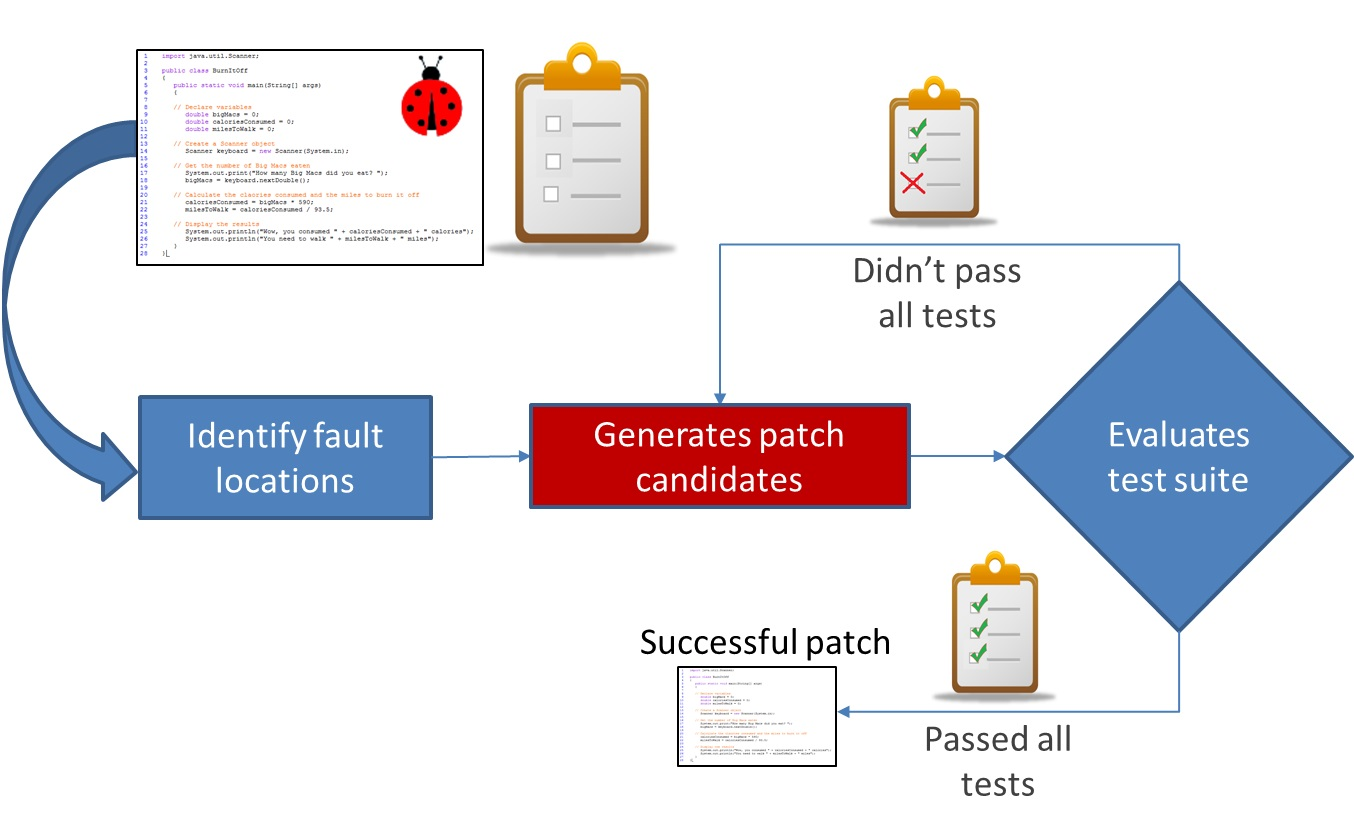
\includegraphics[scale=0.25]{Picture1}
  \caption{Generate and validate approach}
  \label{fig:generateandvalidate}
\end{figure}

Figure~\ref{fig:generateandvalidate} diagrams the basic generate and validate
program repair paradigm. This approach starts with source code that
has one or various bugs to be fixed, and a test suite with passing
test cases that expose expected program behavior that should not change, and failing test 
cases which expose the buggy behavior that should be repaired.  

The first step of this process is to localize the error to a smaller set of
candidate program statements. There is an extensive set of possible approaches
in the fault localization literature that can be adapted to this task
task~\cite{Jones05,Jones02,Chen02,Qi2013}.  A given candidate faulty statement informs
the construction of 
``candidate patches", produced by modifying the program at such a
statement. Candidate patches induce variations of the original program 
that seek to repair the bug in question. To 
create such a candidate patch, these techniques typically identify a subset of
available mutation operators that are applicable to a given location (for
example, such a filter would exclude the insertion of a call to
\texttt{super();} in the middle of a method, as such calls are only legal at the
first line of a constructor). 

Each candidate patch is applied to the input program, which is run on
one or more of the input test cases for evaluation.  If a patch leads the
program to 
pass all the test cases in the test suite, including those originally witnessing
the bug, the candidate patch is presented as a likely repair for the bug. 
If the candidate patch does not pass all the test cases in 
the test suite used to guide the search, the APR
algorithm typically creates more candidate patches 
until it reaches a pre-defined time or variant limit is reached. 

Techniques vary in how they identify and choose between candidate mutation
operators, and how they traverse the search space otherwise. For example, some
mechanisms adapt the manner in which they select candidate patches by assigning
a higher priority to some candidate patches over others based on heuristics~\cite{long16proph};
some others restrict their approach to apply a single edit in the variant
creation process~\cite{Qi13TrpAutoR}; others remove similar patches and prioritize the test cases
according to their likelihood to fail~\cite{Weimer13}; others use various other
random search heuristics, like a random walk~\cite{debroy10} or genetic
programming~\cite{kim2013,legoues12}. 

We discuss other techniques for automatic program repair in
Section~\ref{relatedWork}.

\subsection{Generate and validate mutation operators} 
\label{categorization}

There are a number possible mutation operators that can be applied to a location 
to modify the behavior of a program.  We categorize those used in a cross
section of state-of-the-art techniques into two groups: 

\paragraph{Statement-Edit mutations:}
One family of repair approaches, including GenProg~\cite{legoues12}, 
TrpAutoRepair\cite{Qi13TrpAutoR}, and AE~\cite{Weimer13},
create candidate 
patches by applying coarse-grained mutation operators (such as append, delete, or 
replace) which modify statements of source code to 
repair programs. These prior techniques target the C programming language, where
a statement is grammar nonterminal corresponding intuitively to blocks,
simple statements terminating
with a semicolon or compound statements corresponding to control flow or
loops. In Java, statements conceptually map to program elements expressing
some action to be carried out, including blocks,  while loops, or single-line
method calls. In these approaches, the statements being appended or replaced come from within the project being modified. This is grounded in the notion that source code has a high level or redundancy~\cite{gabel10}.

\paragraph{Template-based mutations:}
Template-based mutation operators describe a family of approaches that instantiate
predetermined templates, more complicated than those in the first family of
approaches, at applicable code locations.  This family includes PAR~\cite{kim2013}, 
SPR~\cite{fan15SPR}, and 
Prophet~\cite{long16proph}.
%
PAR is the product of a study of a large number of 
human 
created patches, from which human annotators abstracted 10 different templates to cover
the most commonly-used changes in bug-fixing practice.
The 10 considered templates are detailed in the top half of Table~\ref{approachTemplates}.

\begin{table}[ht]
  \centering

\begin{tabular}{K{3.1cm}K{5cm}}
\hline 
\multicolumn{2}{C{8cm}}{PAR fix templates} \newline \\
\hline 
1) Null Checker & 6) Parameter Adder and Remover \\ 
2) Parameter Replacer & 7) Expression Adder and Remover \\  
3) Method Replacer & 8) Collection Size Checker \\
4) Expression Replacer & 9) Range Checker\\
5) Object Initializer & 10) Class Cast Checker\\
\end{tabular}\newline \\

\begin{tabular}{K{3.1cm}K{5cm}}
\hline 
\multicolumn{2}{C{8cm}}{PAR extra templates} \newline \\
\hline 
1) Caster Mutator & 4) Lower Bound Setter  \\
2) Castee Mutator & 5) Upper Bound Setter  \\
3) Sequence Exchanger & 6) Off-by-one Mutator\\
\end{tabular}\newline \\

\begin{tabular}{K{3.1cm}K{5cm}}
\hline 
\multicolumn{2}{C{8cm}}{SPR transformation schemas} \newline \\
\hline 
1) Condition Refinement & 4) Insert Initialization \\
2) Copy and Replace & 5) Condition Control Flow Introduction  \\
3) Value Replacement  & 6) Condition Introduction \\
\\
\end{tabular}
  \caption{(Top) PAR fix templates. (Middle) PAR extra templates. (Bottom) SPR transformation schemas.}
  \label{approachTemplates}
\end{table}

In the interest of completeness, we also include six extra templates 
mentioned on the website associated with the Par
approach.\footnote{\url{https://sites.google.com/site/autofixhkust/home/fix-templates}} 
These extra templates provide new mutation operators that helps us compare and
generalize to the other approaches; they are shown in the middle segment of
Table~\ref{approachTemplates} Middle. 
The SPR and Prophet approaches make use of a set of transformation schemas,
shown in the Bottom section of Table~\ref{approachTemplates}.

Some of the SPR/Prophet transformation schema can be seen as a generalization of certain PAR 
templates. For example, \emph{Condition Introduction} can be seen as a superset of 
\emph{Range Checker}, \emph{Collection Size 
Checker}, \emph{Class Cast Checker}, and \emph{Null Checker}. \emph{Condition Refinement} includes \emph{Expression Adder and Remover}. \emph{Insert Initialization} can be 
generalized from \emph{Object Initializer}, \emph{Upper Bound Setter} and \emph{Lower Bound Setter}; \emph{Conditional Control Flow Introduction} can be 
seen as a subset of \emph{Sequence Exchanger};
\emph{Value Replacement} can be seen as a superset of \emph{Method 
Replacer}, \emph{Parameter Replacer}, \emph{Castee Mutator} and \emph{Expression Changer}; and ``\emph{Copy 
and Replace}" can be matched to \emph{Expression Adder}. 

We also considered the program modification tool Kali~\cite{Qi15}, whose
templates correspond to subsets of certain PAR templates their extensions. 
For example, \emph{Redirect Branch} can be seen as
a subset of \emph{Expression Changer}, and \emph{Insert Return} and \emph{Remove Statement} are
subsets of \emph{Expression Adder and Remover} accordingly. In the same way,
many other mutation operators~\cite{Offutt96,Offutt06}, as used in
APR~\cite{debroy10,xuan16} can be seen as subsets of the extensions of the 
Par templates.

To summarize, these approaches have significant similarities between their
included templates.  We have chosen the PAR templates to represent this category 
since these templates provide a more concrete description of how the code is 
changed, enabling replication. As mentioned, 
the SPR, Prophet and Kali templates are represented by one or several of the PAR
templates, but not vice versa.  Finally, the PAR templates naturally target
Java, the subject of our study. 

\section{Building the model} \label{buildingTheModel}

In this section we describe how we mined a probabilistic
model of human bug-fixing edits from a large set of popular Java projects on GitHub. 

\subsection{Selecting the corpus}

We cloned the 500 most-starred Java projects on Github 
as of August 2016. The methodology of 
gathering large,
popular, and active open source Java software repositories is common in
empirical studies (e.g.,~\cite{Ray14}). 
%
We compiled the most recent 100 bug fixing commits per each project. Identifying
bug fixing commits is a difficult
problem in repository mining~\cite{Bird09}. We filter these by applying a
regular expression to the commit message in each of the commits in each of the
projects that looks for words such as ``fix", ``bug", ``issue", ``problem",
etc. following the guidelines by \cite{schroter06,Cubranic05,Fischer03}. 
%
%\\
%\\
%$[Ff]ix(ed|es|ing)?(\backslash s)*([Bb]ug|[Ii]ssue|[Pp]roblem)?(s)?$
%\\
%\\
We included two additional filters in our search: First, we only include commits
that exclusively 
modify Java source code.  Additionally, we restrict our search to commits 
that modify a maximum of three files. We do this to exclude
big merges, such as pull requests or initial commits, and because
large commits are more likely to include changes unrelated to a bug fix~\cite{Dias15,Herzig13,Matsuda15,Kawrykow11}.

\subsection{Identifying mutations in developer commits}
\label{sec:mining}

For each bug fixing commit, we refer to the code before the fix as the
``before-fix" version and the code after as the ``after-fix" version.
We next seek to identify the changes performed between the before-fix and
after-fix versions, to analyze how often they match the mutation operators in
question. 
%
We used two existing tools to identify changes 
between code versions: Gumtree~\cite{falleri14}, a source code tree
differencing framework, and QACrashFix~\cite{gao15}, the tool for generating
fixes via analyzing Q\&A pages.  Specifically, we adapt QACrashFix's
differencing engine, which modifies Gumtree to account for replacements.
These tools create an AST representation of the program files for both the 
before-fix and after-fix representations of the programs for each modified file,
and then use a set of heuristics to match the before-fix version 
with the after-fix version and produce a set of 
changes performed between them. 

For each bug-fixing commit, we then greedily attempt match the identified changes to the
available 
mutation operators. We seek the most complex template that can match a given set
of edits.  For example, to identify
a \emph{Null Checker} application, for each action describing a commit, we check
if the manipualted node
is an \emph{IfStatement}.  If so, we check whether the action
is a node insertion.  If so, we check if the condition in the inserted
\emph{IfStatement} is an 
\emph{InfixExpression} that compares an 
%  An \emph{InfixExpression} as defined by the Eclipse JDT API
% specification has the following form: 
% \\
% \\
% $InfixExpression: \\
% Expression~InfixOperator~Expression
% $
% \\
% \\  
\emph{Expression} to a
\emph{NullLiteral}. If all these conditions are met, we count this sequence of
actions as an instance of a \emph{null checker application}.  These rules are
necessarily heuristic, and we do not claim perfect soundness in our matching,
instead aggregating counted templates over a large dataset.  When a sequence of
actions is matched to a template, it is removed from further consideration (and
thus is only counted as matching a single template).  



%\begin{figure}[!]
%\begin{verbatim}
%var res = 0
%for (ac <- actions) {
%  if(nodeClassName(ac.getNode) 
%    == "IfStatement"){
%      if (actionName(ac) == "Insert"){
%        if((nodeClassName(ac
%          .getNode.getChildren.get(0)) 
%            == "InfixExpression") && 
%              (nodeClassName(ac
%                .getNode.getChildren
%                  .get(0).getChildren.get(1)) 
%                    == "NullLiteral")){
%                      res += 1
%      }
%    }
%  }
%}
%\end{verbatim}
%\caption{Example of heuristic to spot the template Add Null Checker}\label{fig:codeSnippet}
%\end{figure}



\subsection{Two-level probabilistic model for repair}

\begin{figure}[!h]
  \centering
    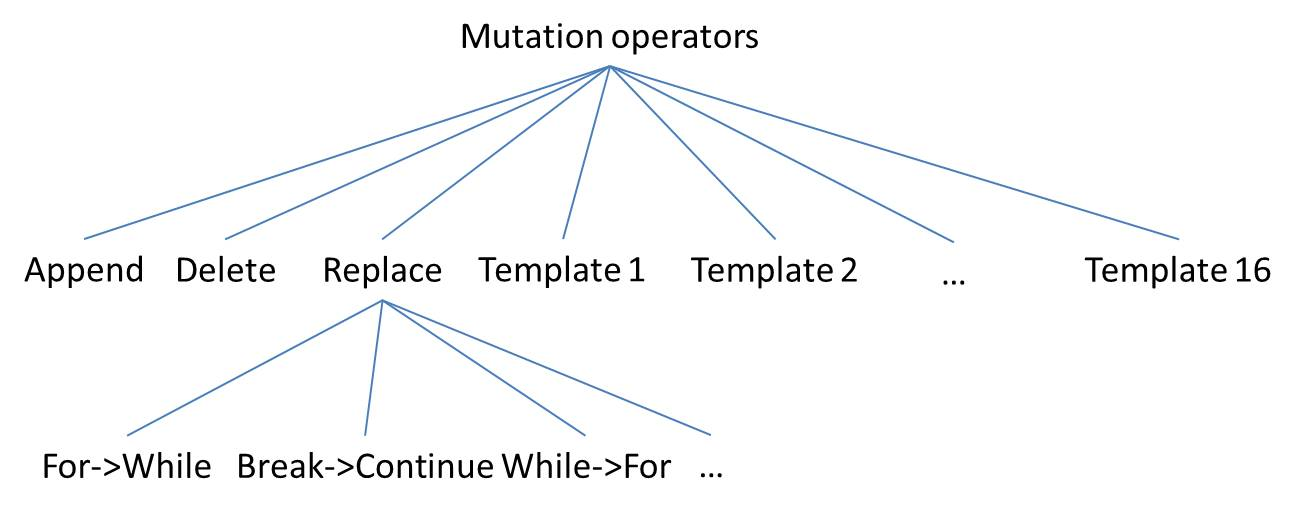
\includegraphics[scale=0.4]{Picture2}
  \caption{Two level probabilistic model}
  \label{fig:probModel}
\end{figure}

We extend an open-source implementation of the GenProg technique adapted for Java
by implementing the mutation operators from
Section~\ref{categorization} as well as a mechanism that allows the tool to
select between the mutation operators according to the probabilities described by
a given model.\footnote{We will release a link to our implementation to support
  a camera ready; we obscure it in the interest of supporting double-blind
  review.}  We construct a two-level model that effectively counts incidences of all considered
mutation operators, and fix code used in replacements  (generalizing prior work
proposing a replacement-only model~\cite{Soto15}):

\paragraph{Mutation operator probabilistic model}
The \textit{Mutation operator probabilistic model} 
describes the probabilities of choosing between the several different mutation 
operators at a particular fault location.
%
To build the \textit{Mutation operator probabilistic model} 
we normalize the number of incidences of each mutation operator observed in our
dataset, matched as described in Section~\ref{sec:mining}.  These normalized
instances comprise a probablistic model, where mutation operator probability is
weighted by its appearance in the dataset.  

\paragraph{Replacements probabilistic model}
If the ``Replacement" mutation operator is 
selected, the \textit{Replacements probabilistic model} model describes the probability of replacing one statement with
another  (referring to the 
``replacee" and ``replacer" statements accordingly), informing the selection of replacement fix code.
%\footnote{https://goo.gl/mMFbnQ
We consider 
the 22 different types detailed by the Eclipse
JDT\footnote{AssertStatement, Block, BreakStatement, ConstructorInvocation, ContinueStatement, DoStatement, EmptyStatement, EnhancedForStatement, ExpressionStatement, ForStatement, IfStatement, LabeledStatement, ReturnStatement, SuperConstructorInvocation, SwitchCase, SwitchStatement, SynchronizedStatement, ThrowStatement, TryStatement, TypeDeclarationStatement, VariableDeclarationStatement, WhileStatement} as
direct known subclasses of the class \texttt{Statement}, and the incidence with which
each 
replaces another. For example: What is the observed incidence of a \texttt{For} loop 
replacing a \texttt{While} loop? Given 22 statement types, any of which may replace one
another, there are 484 possible replacement combinations. 
Note that the observed probabilities are not reciprocal, meaning 
that the probability of a \texttt{For} loop replacing a \texttt{While} loop is different from the 
probability of a \texttt{While} loop replacing a \texttt{For} loop, and the same applies to all 
the different statement types.
This model is built analogously to the
mutation operator model, with a focus on replacer and replacee statement incidence.

\subsection{Multiple edit association rule mining} 
\label{multEdit}

Single-mutation (or single-edit) source code changes are the most 
common subject of analysis in 
state of the art bug-fixing
approaches. This applies to both, approaches that limit the number of source 
code changes they apply to create a program variant to one change per variant 
only (eg, TrpAutoRepair~\cite{Qi13TrpAutoR}, AE~\cite{Weimer13}, Kali~\cite{Qi15}), and 
to approaches whose search space traversal technique can allow multi-edit 
changes (eg. GenProg~\cite{legoues12}, Par~\cite{kim2013}, SPR~\cite{fan15SPR},
Prophet~\cite{long16proph}, etc.) but typically find patches that reduce to
single-edit changes~\cite{arcuri11}.

Although such single-edit patches can be
sufficient to repair non-trivial bugs in real software, many bug fixes in real
software require multiple edits~\cite{zhong15,Soto15}. The combination of possible mutation
 operators to apply in a sequence increases exponentially as we add more source
 code changes, motivating a more precise mechanism to navigate the vast search
 space. 

As a first step towards mitigating this limitation, we propose 
an initial analysis of multi-edit 
source code changes by mining a more expressive model of common changes. In
particular, we are extracting \emph{association rules} between single edit changes 
to model chains of single edit changes, capturing the way humans create them.
Association rules are if/then statements that show relationships between elements in a dataset which happen frequently together.

We use the 
well-known association rule mining algorithm
Apriori~\cite{Agrawal94,Liu98,Zaki2000}, which identifies frequent 
individual items in sets of transactions (commits, in our context).  We extend these sets into 
larger sets that appear often in the transactions, which in our case would be the transactions created 
by each of the commits studied. We have divided our association rule mining to
be built one from each of the models as described in Section~\ref{armRes}. 

To extract association rules from  our data, we
transform each of the mutation operator count and replacement count from 
each of the commits studied into a transaction to be analyzed. A transaction 
in this context is a row of values that describes which mutation operators were applied in a single commit.

Two other basic concepts critical to understanding the Apriori method are the
ideas of \emph{Confidence} and \emph{Support}.
Formally, we define Confidence as:

\begin{center}
$conf(X \implies Y) = \dfrac{supp(X \cup Y)}{supp(X)}$ 
\end{center}

Where X and Y are possible items in a transaction (edit operations in our
context).  Confidence is calculated according to its Support (\emph{supp}, above), 
an indication of how frequently the set of mutation operators (itemset) 
 occurs in the transaction base.
Formally:

\begin{center}
$supp(X) = \dfrac{|\{t \in T; X \subseteq t\}|}{|T|}$
\end{center}

Where X is the itemset and $t$ is each individual transaction in
the database of transactions $T$. Apriori identifies the frequent mutation
operators and replacements that happen together, iteratively extending them to larger
itemsets that appear often in the transactions as identified by these metrics.


\section{Evaluation} \label{evaluation}

We evaluate our model both independently and as part of an automatic repair
technique.  We first evaluate the predictive power of the model by analyzing the
number of correctly predicted mutation operators across a large dataset, using 10 fold cross
validation to mitigate and assess the risk of overfitting
(Section~\ref{sec:generalize}). We evaluate our new APR approach both in a case study 
repair context, to precisely validate the potential increase in efficiency the
probabilistic model affords (Section~\ref{sec:casestudy}), and 
on fifteen real bugs from the Defects4J dataset
(Section~\ref{sec:single}).  Finally, we assess and present the most common 
association rules between mutation operators mined from our corpus
(Section~\ref{armRes}). 

%We also include a section for 
%discussion(Section~\ref{discussion}) and threats to validity (Section~\ref{threatsVal}) 

All experiments are perfomed on a server running Ubuntu 14.04.5 LTS, 
consisting of 16 processors Intel(R) Xeon(R) CPU E5-2699 v3, with 2.30 GHz each
processor, 46080 KB cache each, and 32 GB RAM memory, operating system Ubuntu 
14.04.5 LTS.

\subsection{Model generalization}
\label{sec:generalize}
  

\begin{table}[ht]
\begin{tabular}{llllllllllllllllllllll}
\hline
As & Bl & Br & Cl & Co & Do & Em & EF & Ex & Fo & If \\
0\%&2\%&0\%&2\%&5\%&0\%&0\%&0\%&43\%&0\%&22\% \\
\hline 
La & Re & SC & Ca & Sw & Sy & Th & Tr & TD & VD & Wh \\
0\%&0\%&2\%&2\%&0\%&0\%&3\%&2\%&0\%&19\%&0\% \\
\hline
\end{tabular}
\\
\caption{Example of the Return Statement row of a sub-model created from 
the training data. Replacee probabillities of the replacer ReturnStatement. The acronyms represent the statement kinds detailed in footnote \ref{stmtNames}}
 \label{fig:exPredReturn} 
\end{table} 

First, we evaluate the predictive power of our 
replacements model. Our high-level research question concerns whether 
our mined models are likely to identify the correct fix code across a large
dataset, suggesting its potential utility in a repair context.  To this end, we
compare its predictive accuracy to an \emph{equally distributed} model, in which
the probability of selecting any replacee statement is uniformly random. 
We therefore assess the degree to which each model correctly predicts the
replacer statement for given replacee statements, within the top 5 produced
choices.  Because these models are to be used in the context of program repair,
perfect accuracy (correctness in the Top-1 most likely choice) is unecessary;
however, the noisy search problem induced by fault localization and a larger set
of available mutation operators suggests that a relatively tight bound (top-5)
is likely appropriate.  Additionally, we found obserationally that the top-5
choices serves as a point of inflection between the mined and equal model
performance. 

To mitigate and assess the risk of overfitting and avoid testing and training on
the same data, we use 
10-fold cross validation~\cite{kohavi95} to structure our experiment. 
We segregated the projects that form our corpus into 10 
different folds assigned at random. For each of the 
folds we would take 1 fold for testing and the remaining 9 folds for training a model. 
This is performed 10 times, one time per each fold and then it is 
averaged to see how commonly is the training data able to predict the testing 
data.
We then count the number of testing instances that are correctly predicted 
by the first five guesses from the training sub-model.   

\lstdefinestyle{base}{
  language=Java,
  emptylines=1,
  breaklines=true,
  basicstyle=\ttfamily\color{black},
  moredelim=**[is][\color{red}]{@}{@},
  xleftmargin=20pt, frame=bt, basicstyle={\footnotesize\tt}, numbers=left, keywordstyle=\bfseries, 
	numberstyle=\scriptsize\tt,  moredelim=[is][\color{red}]{@}{@}, deletekeywords={}, captionpos=b, belowskip=1pt, autogobble=true
}

To illustrate the point, consider a simple example. Assume the following
simple bug-fixing patch from our corpus: 

\begin{lstlisting}[frame=single,style=base]
+ if(i > l.size()) {
    return l.get(i); @//original faulty location@
+  }    
\end{lstlisting}

In effect, the developer has replaced the original \texttt{return} with an
\texttt{if-then} statement that wraps it.  Our goal in assessing our model is,
assuming the selected mutation operator 
is \emph{replace}, how often will an \emph{IfStatement} be predicted as the
replacer? If it is returned for the first five instances in a model, the model
correctly predicts this instance.  

Each trained model describes the dataset via
a distribution identifying the (normalized) frequency with which each statement is replaced 
by another. Each combination is described by 
$E_{n,m}$, 
where $n$ is the statement being replaced (replacee) and $m$ the statement it is 
replaced by (replacer).  A predictive model $TP_{n,m}$, $\forall n,m: 1<=n<=22 \land 1<=m<=22$, 
describes how often each statement is replaced by 
other kinds of statements, is trained on the remaining folds. 
Assume for illustration a sub-model $TP_{13,m}$ for return statements shown in Figure~\ref{fig:exPredReturn}.
%
For our example, the most
likely statement chosen to replace a Return Statement according to this row in 
this fictional sub-model would be a Expression Statement (Ex) *$TP_{13,9} = 43\%$). 
The second-most likely candidate is indeed an If statement ($22\%$),
meaning we count this as a correct prediction for this model (as it appears in
the top-5 prediction list). 

To contrast this with the equally distributed approach,
we assign all statements the same probability of being chosen to replace 
a statement under analysis:
$TE_{n,m}$, where $\forall n,m: 1<=n<=22 \land 1<=m<=22 \land TE_{n,m} = 4.54\%$. 
For the top five choices in a prediction scheem, we choose five uniformly choices at
random for each prediction. 

%For example, if the approach picks at random the statements: Assert Statement 
%$TE_{13,1}$, 
%Do Statement $TE_{13,6}$, Expression Statement $TE_{13,9}$, Throw Statement 
%$TE_{13,18}$ and Try Statement $TE_{13,19}$. Then we 
%would match how many of the instances in the testing data were correctly 
%predicted by this equally distributed schema.

%In this example, the 4 instances of Expression Statement $E_{13,9} = 4$, the 
%instance of Do 
%Statement  $E_{13,6} = 1$, and the instance of Try Statement $E_{13,19} = 1$ 
%would be considered to be correctly 
%predicted; while the 2 instances of If Statement $E_{13,11} = 2$, and the 2 
%instances of 
%Continue Statement $E_{13,5} = 2$ would be considered to be incorrectly 
%predicted. Since the 
%equally distributed approach in this example correctly guessed 6 out of 10 
%instances of the testing data, we would then say that in this particular case, 
%the equally distributed approach correctly predicted 60\% of the instances in 
%the testing set.  


\begin{table}[ht]
\begin{tabular}{l|rr|rr|rr}
   &\multicolumn{2}{c|}{Replacements} &\multicolumn{2}{c|}{Mutations}&\multicolumn{2}{c}{Instance count} \\
   	\hline
Test fold	&Prob&	EqDist&Prob&	EqDist & Replac  & Mut\\
	\hline
1	&70\%&	25\% &  95\% & 64\% & 155 &17313 \\
2	&100\%&	25\%  & 93\% & 63\% & 86 & 17232 \\
3	&82\%	&23\% & 95\% & 81\% & 81 & 16754\\
4	&81\%	&40\%  & 94\% & 9\% & 101 & 14159 \\
5	&90\%	&27\%  & 95\% & 2\%& 99 & 17022 \\
6	&84\%	&21\%  & 95\%& 58\%& 75 & 14945 \\
7	&86\%	&24\%  & 93\%& 7\%& 79 & 12901 \\
8	&96\%	&23\%  & 95\%& 27\%& 55 & 10552 \\
9	&88\%	&8\%  & 93\%& 62\%& 82 & 14568\\
10	&100\%	&31\%  & 95\% & 6\%& 116 & 19140\\
	\hline
Mean	&87.7	&24.70  & 94.3 & 37.9 & \\
	\hline
Variance	&87.12&	64.23  & 0.90 & 929.87 & \\
	\hline
Std dev	&9.33&	8.01  & 0.94 & 30.49 & \\
	\hline
Aggregate& 877 & 247 & 943 & 379 & 929 &  154586\\


\hline
\end{tabular}
\center
  \caption{Correctly predicted percentage according to 10 fold cross
    validation. The replacement probabilistic model (left) is able to predict
    the correct statement kind to replace a faulty one in 87\% of the times,
    this is an improvement of almost a factor of 4 when compared to the equally
    distributed model. The mutations model(middle) is able to predict the
    correct mutation to be applied almost by a factor of 3 when compared to the
    equally distribured.} 
  \label{tab:results10fcv}
\end{table} 

\todo{Fill out the missing values in the table III}

\todo{Exlpain the last two columns in the text and caption}
%\begin{figure}[!h]
%  \centering
%    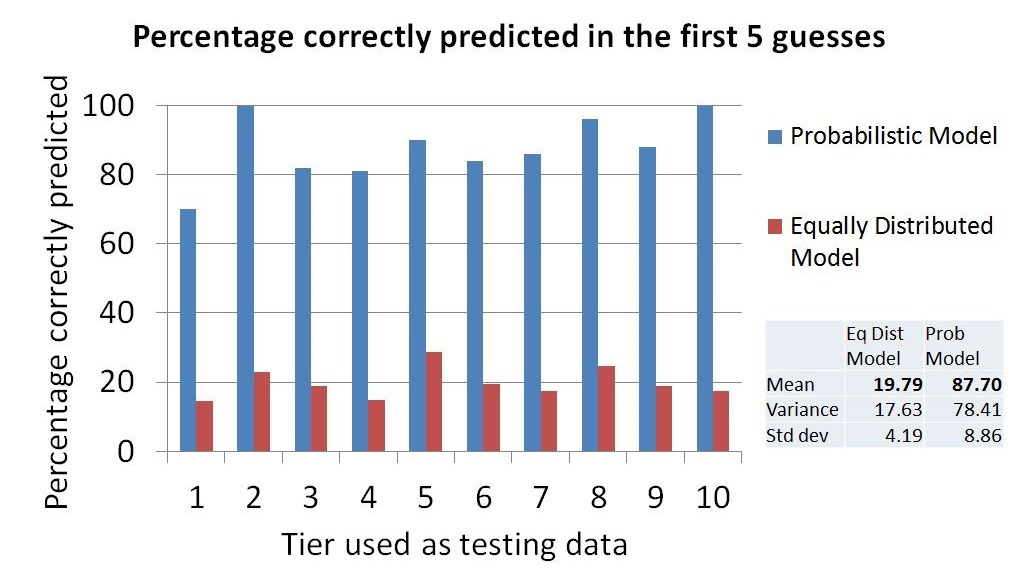
\includegraphics[scale=0.33]{sanity1}
%  \caption{   }
%\end{figure}
The results of this evaluation over all 10 folds are detailed in
Table~\ref{tab:results10fcv}. For each fold, we show the percentage of correctly 
predicted instances of the testing data in each particular fold by the top five
guesses of the equally distributed approach for the replacements model. The
fourth and fifth columns show the percentage of correctly predicted
instances using the top five  
guesses of the sub-model of each of the folds for the mutations model. Finally the sixth and seventh columns are the number of instances in each of the folds. We have a difference of 63\% between the means of the two models in the replacements model, and a difference of 56.4\% between the mean values of correctly predicted instances in the probabilistic and equally distributed models for the mutations model.

\subsection{Case study}
\label{sec:casestudy}


\begin{figure}[t]
\begin{lstlisting}[frame=single,style=base]
  public int mid(int x, int y, int z){
    int ret = z;  
    if(y<z){
      if(x<y){
        ret = y;
      }else if(x<z){
        ret = z; @//bug, it should be ret=x;@
      }
    }else{
      if(x>y){
        ret = y;
      }else if(x>z){
        ret = x;
      }
    }
    return ret;
  }	
	\end{lstlisting}
	\caption{Source code of an independent example. The bug to be fixed is annotated and highlighted}
	\label{fig:initialExample}
\end{figure}

We assess our
models' utility in a repair algorithm on a small case study example, constructed
to differ from the code used in the model.  Consider the buggy method shown in
Figure~\ref{fig:initialExample}, which is intended to  calculate the median 
of three numbers.  The incorrect line reads 
$ret = z;$ instead of $ret = x;$. There is one failing test case and eigth passing test cases that describe the inputs and expected outputs of the method.

We run our implementation of the GenProg approach targeting Java and using the
equally- and probabilistically-constructed models to select between statement kinds in the replacements model. \todo{But not the replacement model for replacements? RESPONSE: Opposite, we ran it with the replacements model. At this point the mutations model didn't exist. So we run it with replacement only to show how the replacements work if the only option is replacement. And the second case, we let it pick between three mutations using the normal genprog way of picking mut ops and when it picks replace, it uses the replacements model. We started with this, and then up'ed the level to the mutations model}\todo{Also, in
  the next subsection you say you build the full model on 500 projects.  If
  that's true, what is this model built on? RESPONSE: The one we used here was built from 200. I wrote somewhere here that we tested this case study with a subset of the model, but that phrase probably got removed. Should I put it back again? RESPONSE: YES.  Please just do things like this without asking; clearly it's confusing to me.  That's why I asked.  You don't need my permissino to put basic facts in.}
In the interest of sanity checking our approach, we 
start by evaluating on a restricted subset of 
the mutation operators: (1) Only using the $Replace$ mutation operator, and (2) Using only $Append,~
Delete~and~Replace$ operators.  We measure the average number of variants
evaluated before finding a repair, a machine- and test-suite independent proxy
for time. We set the size for each population to 40, we ran 20
seeds per trial, with a timeout of 4 hours for each run.  We average results of 10 random trials.

In the results shown in Table~\ref{fig:resultsReplace} Left, we consider only the mutation operator 
$Replace$, which means that the tool will disregard all other mutation 
operators and will only apply Replace operations using the probabilistic model 
of Replacements. This is because at this step we are evaluating our model in a 
subset of the mutation operators to understand if it makes sense to move forward and 
continue implementing the rest of the mutation operators.
%
In this Table we can analyze the average, standard deviation and success rate of an automatic program repair tool running 10 different seeds, contrasting the 
number of variants it takes to find a patch using the probabilistic approach, with the number of variants it takes to find a patch using the 
equally distributed approach 
%
As we can derive from the graph, the probabilistic approach was able to find a 
patch faster than the equally distributed for all the seeds tested. On average,
we found that by using the probabilistic model we  
could find a patch in 23.8 variants, while it took an average of 60.5 variants 
to find a patch using the equally distributed model.

\begin{table}[ht]
\begin{tabular}{l|rr|rr}
  & \multicolumn{2}{|c|}{Replace only} & \multicolumn{2}{c}{Append,Remove,Replace} \\
\hline
\textbf{Seed}& Avrg & StdDev & Avrg & StdDev\\
\hline
\textbf{Prob} & 23.8 & 24.8  & 22.6 & 23.7  \\

\textbf{Eq Dist} & 60.5 & 57.1 & 41.4 & 41.2 \\
\hline
\end{tabular}
\\
\\
\center
  \caption{Number of variants it takes to find a patch using different sets of
    mutation operators to guide the search for a patch of the case study using
    only Replace and Using Append, Remove and Replace operators. Random success
    rate for all experiments is 100\%. }
  \label{fig:resultsReplace}
\end{table} 

%\begin{figure}[!h]
%  \centering
%    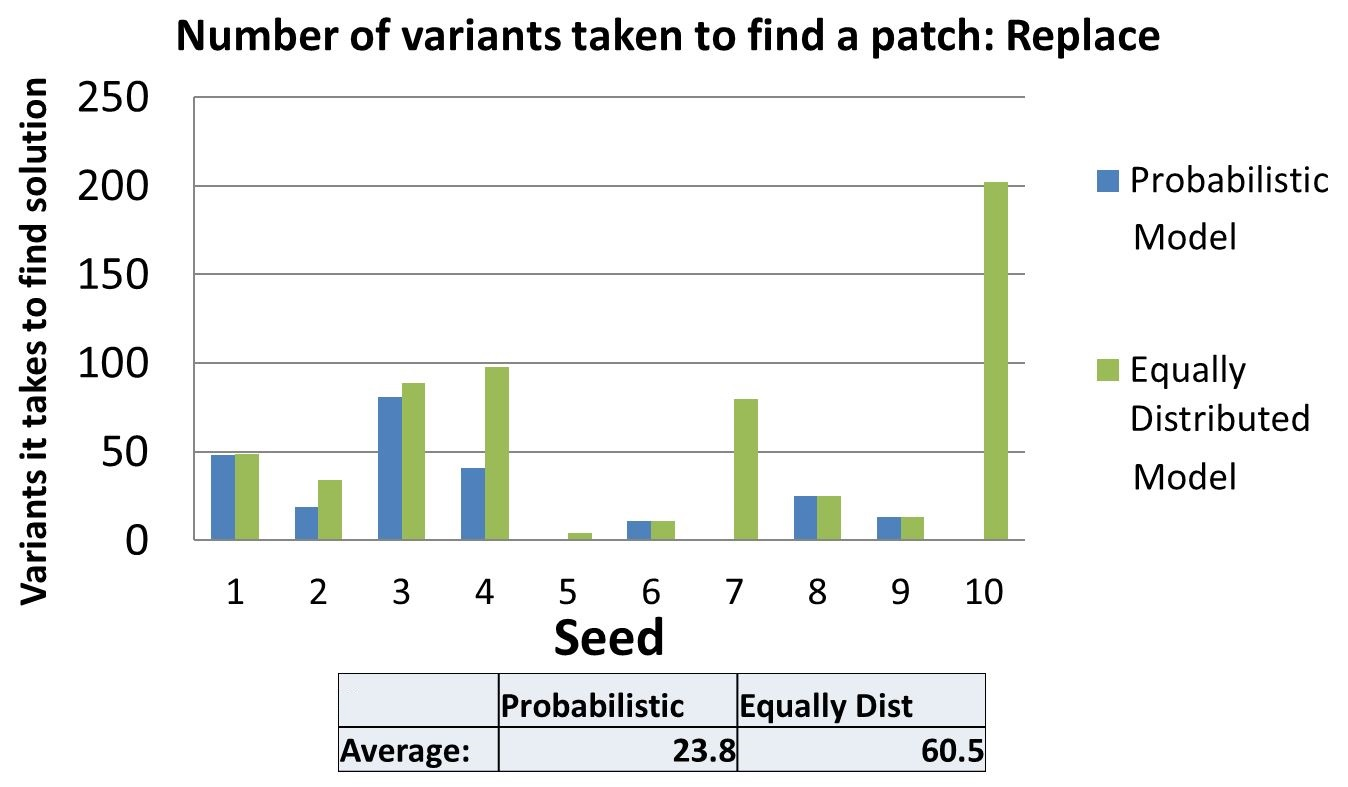
\includegraphics[scale=0.25]{sanity3}
%  \caption{Using replace to guide the search for a patch of the case study}
%  \label{fig:resultsReplace}
%\end{figure}

In Table~\ref{fig:resultsReplace} Right, we consider three mutation operators: Append, 
Remove and Replace. In this case the data 
shows that using the probabilistic model we obtain a mean of 22.6 variants 
before finding the patch, while it takes an average of 41.4 variants to find the 
patch using the equally distributed approach. In both experiments, the
probabilistic model outperformed the equally distributed model on every seed.

\subsection{Single line bug repair}
\label{sec:single}

\begin{table*}\centering
\begin{tabular}{r|rr|rr|rr|rr|rr|rr}
\toprule
  &\multicolumn{4}{c|}{\textbf{Stmts Only}} & \multicolumn{4}{c|}{\textbf{Templates}} & \multicolumn{4}{c}{\textbf{All}} \\  
  & \multicolumn{2}{c|}{\textbf{Equally Dist}} & \multicolumn{2}{c|}{\textbf{Probabilistic}} & \multicolumn{2}{c|}{\textbf{Equally Dist}} & \multicolumn{2}{c|}{\textbf{Probabilistic}} & \multicolumn{2}{c|}{\textbf{Equally Dist}} & 
\multicolumn{2}{c}{\textbf{Probabilistic}} \\

 \textbf{Bug Name} & \textbf{Time} & \textbf{Quality} &  \textbf{Time} & \textbf{Quality} &  \textbf{Time} & \textbf{Quality}&  \textbf{Time} & \textbf{Quality}&  \textbf{Time} & \textbf{Quality}&  \textbf{Time} & \textbf{Quality} \\\midrule

 Closure \#10 & {221.0}& {100\%} & {179.5} &{100\%} & {175.1}&{100\%} & {121.3}&{100\%} & {163.3}&{100\%} & {157.4}&{100\%} \\

 Closure \#18 & \multicolumn{2}{c|}{Not found} & \multicolumn{2}{c|}{Not found} & {36.2}&{100\%} & {197.5}&{100\%} & {45.0}&{100\%} & {139.0}&{100\%} \\

 Math \#2 & \multicolumn{2}{c|}{Not found} & \multicolumn{2}{c|}{Not found} & {109.4}&{0\%} & {39.6}&{0\%} & {109.4}&{0\%} & {39.6}&{0\%} \\

 Time \#19 & {94.1}&{100\%} & {80.7}&{100\%} & \multicolumn{2}{c|}{Not found} & \multicolumn{2}{c|}{Not found} & {135.1}&{100\%} & {91.9}&{100\%} \\

 Chart \#1 & {1.8}&{0\%} & {7.3}&{0\%} & {4.9}&{0\%} & {19.0}&{0\%} & {2.2}&{0\%} & {4.8}&{0\%} \\

\bottomrule
 
\end{tabular}
		\caption{Repair success of various models for three different operator
          sets.  For each, we report time in terms of variants evaluated to a
          repair (Time) and percentage of produced patches that pass of all of a
          held-out second test suite. \label{tab:singleLineBugs}}
\end{table*}

In this subsection, we evaluate the success of automatic program repair with our
model on real-world bugs  by comparing the performance of our 
automatic program repair tool using the probabilistic model to one using the
equally distributed model.  
We built the whole model with 500
projects in Github with the most stars.
 This is to generate the largest code base so far to the best 
of our knowledge, surpassing all the previous state of the 
art~\cite{long16proph,Soto15,zhong15,martinez15,xuan16}. 
In these experiments, we include all mutations described in
Section~\ref{categorization} (in our dataset, Template-Based mutations comprise 29.26\% of the corpus; Statement-Edit mutations make up 70.74\% of the 
corpus).

\subsubsection{Repair results}

We consider for repair a subset of the Defects4j~\cite{just14}
benchmark, a database and extensible 
framework of real bugs that enables reproducible studies in software testing 
research. This database currently contains 395 real bugs from 6
open source programs,\footnote{Note that we initiated this study when Defects4J
  contained 5 subjects, and thus have no bug instances from the recently-added
  Mockito project.} along with developer-provided test suites, cases that
expose each bug,  and
corresponding developer-provided patches. Defects4j has been previously used
in evaluating previous work in APR~\cite{Durieux15}.
In keeping with APR's typical focus on smaller patches, we
restrict attention to the first 3 bugs from each project that required a 
single line edit: Chart 1, 
Chart 8, Chart 20, Closure 10, Closure 14, Closure 18, Lang 6, Lang 16, Lang 21, 
Math 2, Math 5, Math 10, Time 4, Time 16 and Time 19.
To diminish the degree of randomness in this experiment and control for the
effect of the mutation probabilities specifically,  we manually
set fault localization for each bug.  This controls for inefficiency and noise
in fault localizaiton. Anecdotally, we observe that less-accurate fault localization increases the amount of
time taken to repair these defects, as expected (results not shown). 

We set the size for each population to 40 for consistency with 
previous work~\cite{legoues12,kim2013}, we ran 20
seeds per trial, 10 generations, a timeout of 4 hours for each run, in keeping with 
recommendations on the assessment of stochastic techniques~\cite{arcuri11}.
To compare the efficacy of different types of mutation operators,
we tested three operation sets: (1) Statement-Edit mutations only (2) Template-based mutations 
only (3) All mutations.  

We assess number of variants to a repair (as in
Section~\ref{sec:casestudy}).  Additionally, as a proxy for patch quality (to
mitigate the risk of plausible but as yet incorrect patches~\cite{Qi15}), we
evaluate patches using held-out test suite~\cite{legoues2012,Smith15} by automatically building a second
test suite that independently describes the same behavior as the test suite that
guides the search process. We use Randoop~\cite{pacheco07}, an established
automatic test suite generation tool for Java, to generate this second test
suite. 
For each successfully-patched bug, we 
run Randoop for ten minutes (six times the default value) on the human-patched
version of the code.\footnote{We will release our test suites post-review.}  We
thus additionally report patched program success on these independent test
suites. 

Our modified APR techniques patched 5 of the 15 bugs, as shown in 
Table~\ref{tab:singleLineBugs}. In the first row of Table~\ref{tab:singleLineBugs} (Closure \#10) we can see
that in all three comparisons (Statement-Edit Only, Template-Based Only, and All
mutations), the probabilisitc model outperforms
the equally distributed model. This happens as well for
Math \#2 and Time \#19 except for the cases where no patch was
found. By contrast, for bugs Chart \#1 and Closure \#18, the equally
distributed approach finds a patch faster on average. This is due to the fact
that these bugs are patched with a mutation that is rare to apply by developers,
therefore it is more likely that the mutation operator will be chosen by randomness
than by an informed model trying to replicate how developers behave.

Our results also show that considering all available mutation operators is
preferable to 
restricting the mutation operator pool to just one of the categories. For the
Statement-Edit category: 3 out of 6 were fixed faster when combining it with
Template-Based mutations, and 3 out of 6 were slower. For the Template-Based
category: 4 out of 8 were fixed faster when combining it with Statemtent-Edit
mutations, 2 out of 8 were the same, and 2 out of 8 were slower. This suggests
that the expressive power afforded by an increased set of operators may
outweight the commensurate increase in search space size, though it is safe to
assume that this benefit must be supported by sufficiently accurate fault
localization. 

Table~\ref{tab:singleLineBugs} also shows the results of evaluating our patches
on the second, held-out test suites. We noticed a
constant behavior regarding the different sets of mutations. In this sample, if
a model is able to find a patch faster, this appears independent of the mutation
set.  We also notice that
the quality of patches produced  appears constant, and unaffected by model:
either the tool produces patches in 
that all pass the second test suite, or it produces patches that do not. 
%\subsection{Bugs fixed with a multi line edit within a function}
%Last evaluation with the bugs we found had a fix

\subsubsection{Repair example} \label{examPatches}

\begin{figure}[t]
\begin{lstlisting}[frame=single,style=base]
LegendItemCollection result = 
  new LegendItemCollection();
if (this.plot == null) {
  return result;
}
int index=this.plot.getIndexOf(this);
CategoryDataset dataset = 
  this.plot.getDataset(index);
@-if (dataset != null) {
 - return result;
-}@
int seriesCount=dataset.getRowCount();
	\end{lstlisting}
	\caption{A snippet of the source code of the Chart 1 bug fixed using the
      probabilistic model. The APR tool with the probabilistic model deleted code similar to what the
      developer did.\label{fig:chart1.1}}
\end{figure}

\begin{figure}[t]
\begin{lstlisting}[frame=single,style=base]
LegendItemCollection result = 
  new LegendItemCollection();
if (this.plot == null) {
  return result;
}
int index=this.plot.getIndexOf(this);
CategoryDataset dataset = 
  this.plot.getDataset(index);
@+ if (dataset != null) { 
 + this.itemLabelGeneratorList=new ObjectList();
 + this.toolTipGeneratorList=new ObjectList();
 + this.urlGeneratorList=new ObjectList();
 + this.legendItemLabelGenerator = 
 +  new StandardCategorySeriesLabelGenerator();
 + this.backgroundAnnotations=new ArrayList();
 + this.foregroundAnnotations=new ArrayList();
 + }@
int seriesCount=dataset.getRowCount();
	\end{lstlisting}
	\caption{Source code of Chart 1 bug fixed using the equally distributed
      model. The APR tool inserted code unlike a developer would have done it by
      allocating global variables that may be used later.\label{fig:chart1.3}}

\end{figure}


In this subsection, we provide example patches produced using the alternative
models, as compared to a human patch.  Consider the snippet of code corresponding
to the first Chart bug (and its developer fix) from the Defects4J dataset
(Figure~\ref{fig:chart1.1}).  The developer patches this bug by deleting the if
statement.  The mined statement-level mutation model favors deletion, and thus
our repair efforts found patches that removed either the entire \texttt{IfStatement}, or its body (line 9).
By contrast, the equally-distributed model has a higher probability of leading
to a patch such as the one shown in Figure~\ref{fig:chart1.3}.  This test case
passes when, in the case that \texttt{dataset} is not null, nothing is returned;
this patch avoids this, but also allocates state variables that are not
necessary at present (and whose state may have unknown effects in other
executions). 

\subsection{Association Rule Mining} \label{armRes}

We mined our corpus using the Association Rule Mining algorithm Apriori 
to find rules of mutation operators and 
replacements that happen commonly together, which will give us a hint regarding
what mutation operations and replacements can be applied together to form multi-edit
source code changes.

\paragraph{Mutation operator rules:}
To create these association rules among several mutation operators, we mine the
transactions made out of the commits created by humans in the corpus of projects
studied and we look for rules that have at least 90\% Confidence, where
Confidence is an indication of how often the rule has been found to be true.  
These rules are ranked by their confidence; in this case, the top 10 rules shown
below have a confidence of a 100\%, meaning that in 100\% of the cases
studied, every transaction that showed the antecedent also showed the consequent.
They are obtained with a 1\% support, which means that each of these rules
individually appear in at least a 1\% of all the transactions of the overall
corpus. We show the top ten association rules for the mining of single edit 
mutation operators to indicate the structure of the rules; and release all mined
rules with over 90\% Confidence and 0.1\% Support:\footnote{We 
  will link the full list of mined association rules post double-blined
  review.} 

%Minimum support: 0 (1 instances)
%Minimum metric <confidence>: 0.9
%Number of cycles performed: 20
\begin{itemize}
\item Replace \& Delete $\implies$ Append
\item Delete \& AddNullCheck $\implies$ Append
\item Replace \& SeqExchanger $\implies$ Append
\item Replace \& ParamReplacer $\implies$ Append
\item Delete \& CasteeMutator $\implies$ Append
\item Replace \& Delete \& ParamReplacer $\implies$ Append
\item Replace \& AddNullCheck $\implies$ Append
\item Replace \& Delete \& SeqExchanger $\implies$ Append
\item Delete \& ExpressionAdder $\implies$ Append
\item Delete \& AddNullCheck \& ParamReplacer $\implies$ Append
\end{itemize}

Append is the most common single edit mutation operator applied by developers. This behavior is
reflected in the fact that it is the consequent in the all the top ten mined
rules.  
%\footnote{https://goo.gl/UT8QbI} 
%REPLACE FOR CAMERA READY: https://github.com/mausotog/ReplacementsEmpiricalStudy/blob/master/ResultsAssociationRuleMiningMutOperators.txt

\paragraph {Replacement rules} We have also analyzed association rules for the
replacements model, obtaining
the following rules with a 0.01\% Support and 90\% Confidence.
The ten best rules we found are:
%Minimum support: 0.0001 (1 instances)
%Minimum metric <confidence>: 0.9
%Number of cycles performed: 20
\begin{itemize}
\item Block replaces ReturnStatement \& ExpressionStatement replaces IfStatement $\implies$ Block replaces IfStatement
\item VariableDeclarationStatement replaces AssertStatement $\implies$ SwitchCase replaces BreakStatement
\item EnhancedForStatement replaces TryStatement $\implies$ ExpressionStatement replaces ReturnStatement
\item ForStatement replaces TryStatement $\implies$ ExpressionStatement replaces VariableDeclarationStatement
\item VariableDeclarationStatement replaces EnhancedForStatement $\implies$ ExpressionStatement replaces VariableDeclarationStatement
\item VariableDeclarationStatement replaces ForStatement $\implies$ ExpressionStatement replaces VariableDeclarationStatement
\item ForStatement replaces TryStatement $\implies$ IfStatement replaces TryStatement
\item VariableDeclarationStatement replaces ForStatement $\implies$ ForStatement replaces TryStatement
\item ForStatement replaces TryStatement $\implies$ VariableDeclarationStatement replaces ForStatement
\item VariableDeclarationStatement replaces ForStatement $\implies$ IfStatement replaces TryStatement
\end{itemize}

%Similar to the one described above, the authors have made available the full list of association rules with over 90\% Confidence and 0.01\% Support.\footnote{https://goo.gl/omk60t}
%REPLACE FOR CAMERA READY: https://github.com/mausotog/ReplacementsEmpiricalStudy/blob/master/ResultsAssociationRuleMiningReplacements.txt

\subsection{Threats to Validity} \label{threatsVal}

\noindent\textbf{Internal validity:}
Regarding possible errors in our implementation and experiments, to run our
comparison with Genprog, we used an open-source implementation of GenProg
targeting Java. We release our code, as well as our templates,
independently-generated tests, and mined models for scrutiny and extension by other
researchers, to mitigate the risk of errors in our implementation or approach. 
%REMOVE THIS FOR CAMERA READY
%in the project mentioned before 

\noindent\textbf{External validity:} 
Regarding the generalizability of our findings, it is possible 
that our results will not generalize external datasets and further
real life bugs. To mitigate this concern, we evaluate 
on a state of the art bug-mining including bugs from well-known open-source
pograms, covering a diversity of applications, and distinct from the dataset
from which the models were mined.  We also use 10-fold cross validation in
assessing our model, to reduce the risk of training and testing on the same
data.  

The authors acknowledge the risk of producing bad quality patches that would not generalize
to a different description of the behavior the program should have. We attenuate this by 
assessing the quality of the generated patches with a held-out test suite.
There is risk in the fact that we are manually giving the
faulty location to the APR tool, since APR tools do not know in advance what the 
fault location is. This is for the purposes of evaluating the patch creating process
only without the noise that fault localization might introduce.

\noindent\textbf{Construct validity:}
Regarding the suitability of our evaluation metrics, we evaluate patch
quality by running the generated patches on a second test suite created
from a human patch, which is to a certain extent a biased measure since we can
not guarantee that the human created patch is perfect. Nevertheless, we consider this to be a
best known practice, since this way we provide an alternative to subjectively asking a biased human developer
whether he/she considered the patch to be correct or not. 

\section{Related Work} \label{relatedWork}

There have been previous efforts to create a model based on human behavior.  Soto et al.~\cite{Soto15} 
built a probabilistic model to model the replace mutation 
operator only, based in 
an instance count of each statement type using the platform 
BOA,~\cite{dyer2013}.  They do not evaluate the model in the context of a repair
tool.  
HDRepair~\cite{xuan16} 
uses fix history
to help assess patch suitability and fitness in the context of a genetic
programming search strategy. The fitness of the generated
fix candidates is determined by the frequency with which the changes included in
a given patch occur in the corpus using a Graph-based representation of the bug
fixes.  Similary, Prophet~\cite{long16proph} uses a
probabilistic model of a subset of our considered mutation operators built on 
the history of 8 different projects. This model is used to rank candidate
patches for evaluation.  Our approach follows this intuition to mimic human
behavior; unlike the previous work, we apply this knowledge when actually
creating patch candidates rather than when evaluating them.  

Zhong and Su~\cite{zhong15} perform an empirical study of
real bug fixes on six projects, studying the incidence of three mutation
operators, among other questions about the applicability of APR.  Martinez and
Monperrus~\cite{martinez15} similarly study mutation operator incidence across 14 
projects. Our work considers a broader set of
mutation operators over a larger corpus, the largest, to the best of our
knowledge, studied in existing work. In 
order to counter the 
risk of overfitting to a small set of training projects as performed before, our 
current study trains the model over 500 projects, covering a diversity 
of domains.

Par~\cite{kim2013} describes a manual set of 10 templates of common behavior to
create patches, showing that such templates result in patches of higher
human-adjuded acceptability than statement-edit-based patches.  Our study takes into consideration a superset
of these templates, provides steps towards
accounting for multi-edit source code changes, an understudied problem, and,
importantly, mines and models these operators and their incidence automatically
(rather than manually).

There exist a broad array of APR techniques proposed, especially recently; we
survey many of them in Section~\ref{background}, focusing on heuristic or
syntactic generate-and-validate techniques.  Semantic-based techniques use
semantic analysis or reasoning~\cite{nguyen13,mechtaev15,Mechtaev2016}, or
semantic search~\cite{ke15} to construct candidate patches.  Similarly,
synthesis based repair is a family of techniques that uses constraints to build
patches following the description of the constraints. These constraints may be
specifications created by developers, formal verification, invariants,
etc.~\cite{jin11,wei10}.  Such techniques typically use synthesis to construct
repairs, with a different mechanism for both constructing and traversing the
search space, and our approach is thus less immediately applicable.
 

\section{Conclusion} \label{conclusion}

In this paper, we analyze the way in which current state of the art automatic 
program repair approaches select mutation operators to create candidate 
patches. We analyze, categorize and compare the mutation operators being used by 
state of the art approaches. We analyzed the last 100 bug fixing commits from the
500 most-starred Java projects on Github, which is the largest corpus analyzed
to date, to the best of oour knowledge.  We created a two-level probabilistic model describing
the likelihood of selecting bug-fixing mutation operators, according to the
observed incidence of their use by human developers. 

We evaluated our single-edit approach in several ways: by performing an internal evaluation of 
its predictive power (using 10 fold cross 
validation), by comparing the equally distributed model with the probabilistic
 model on an initial case study; and finally by comparing the two models 
 by running them on 15 bugs using the database of bugs and extensible 
framework Defects4j. For these bugs, we measured the number of variants it takes to find the 
patch as well as the quality of produced patches, using a second automatically-created test suite.
Note that in \ref{tab:singleLineBugs}, for two bugs,
the equally distributed model performed better than the probabilistic
model. In these cases, unusual mutation operators were involved in the repair. 
We also notice that applying different probabilities when constructing variants
does not make the patches found in either of the models more likely to pass a
second test suite for these five bugs. Further evaluation should be performed to
determine if one of the models creates higher quality patches than the other. 
Overall, however, we found that automatic program repair appears to benefit
from having a diverse mutation operator pool containing mutation operators from both categories,
rather than restricting their choices to just one category, increase in search
space size notwithstanding; future improvements in fault localization thus will
serve to further benefit from more precise models of mutation selection. 

We also constructed a set of association rules that describe 
how often different sets of mutation operators can predict the change that will 
come next and how often subsets of mutation operators are applied together.
Note that there is a tension between the Support and the Confidence in our transaction 
base, in which we 
evaluate the different mutation operators being applied to source code in bug 
fixing commits. 
If we increase the Confidence and decrease Support, we obtain rules such that
the antecedent and consequents always occur to gether.  This may produce rules that
do not occur often, but, when they \emph{are} selected, are very likely to be
correct. n the other hand, if 
we increase the Support and decrease the Confidence we would obtain rules that 
are guaranteed to happen in a certain percent of the corpus, which means, that 
the relationship described by the rules, happen often, but confidence is 
sacrificed, which means that there will be a higher percentage of the 
transactions in which the antecedent is present, but the consequent is not. 

Finally, we have analyzed a field that has been understudied in the past and which covers 
the vast majority of bug fixes in software systems, which is Multi-edit source code changes. 
We have created a set of association rules using Apriori, a state of the art
methodology for association rule mining based on the analyzed corpus. Our
initial analysis of how single-edit source code changes can be chained together 
to become multi-edit source code changes by following human behavior provides a
first step towards an efficient mechanism for traversing the large search space
of multi-edit repairs.



% conference papers do not normally have an appendix


% use section* for acknowledgment
\section*{Acknowledgments}
The acknowledgments section will be added for the camera ready version. 





% trigger a \newpage just before the given reference
% number - used to balance the columns on the last page
% adjust value as needed - may need to be readjusted if
% the document is modified later
%\IEEEtriggeratref{8}
% The "triggered" command can be changed if desired:
%\IEEEtriggercmd{\enlargethispage{-5in}}

% references section

% can use a bibliography generated by BibTeX as a .bbl file
% BibTeX documentation can be easily obtained at:
% http://mirror.ctan.org/biblio/bibtex/contrib/doc/
% The IEEEtran BibTeX style support page is at:
% http://www.michaelshell.org/tex/ieeetran/bibtex/
%\bibliographystyle{IEEEtran}
% argument is your BibTeX string definitions and bibliography database(s)
%\bibliography{IEEEabrv,../bib/paper}
%
% <OR> manually copy in the resultant .bbl file
% set second argument of \begin to the number of references
% (used to reserve space for the reference number labels box)
%\begin{thebibliography}{1}

%\bibitem{IEEEhowto:kopka}

%\end{thebibliography}

\bibliographystyle{abbrv}
\bibliography{sigproc}  % sigproc.bib is the name of the Bibliography in this case
% You must have a proper ".bib" file
%  and remember to run:
% latex bibtex latex latex
% to resolve all references



% that's all folks
\end{document}


